\documentclass[portrait]{seminar}
%\usepackage{pandora}
\usepackage{color}
\usepackage{fancybox}
\usepackage{alltt}
\usepackage{epsfig}
\usepackage{rail}
\usepackage{bar}
\usepackage{url}
\usepackage{rotating}
\usepackage[normalem]{ulem}
\usepackage{latexsym}
\usepackage{amsmath}

\begin{document}

\boldmath
\newcommand{\RA}{$\rightarrow$}
\newcommand{\LL}{\mbox{$[$\hspace{-0.15em}$[$}}
\newcommand{\RR}{\mbox{$]$\hspace{-0.15em}$]$}}
\newcommand{\CC}[1]{\mbox{\tt $\LL$#1$\RR$}}

\slideframe{shadow}

%%% Activate one of these to get either Aarhus style or McGill style 
%%% by putting a #1 in the appropriate line.
\newcommand{\mcgill}[1]{#1}
\newcommand{\aarhus}[1]{}

%%% Define this to be the name of your term
\newcommand{\courseterm}{Fall 2012}




\aarhus{
\newpagestyle{dOvsstyle}{dOvs'98 Week 44 \hfil Virtual machines}{\hfil \thepage}
}

\mcgill{
\newpagestyle{dOvsstyle}{COMP 520 \courseterm  \hfil Virtual machines (\thepage)}{}
}
\slidepagestyle{dOvsstyle}

\begin{slide*}
\begin{tabbing}
\aarhus{{\Large\bf Week 44}}\\
~\\
{\Huge\bf Virtual machines}\\
\end{tabbing}
\vfil
\end{slide*}

\begin{slide*}
Compilation and execution modes of\\
Virtual machines:\\

\begin{center}
\setlength{\unitlength}{0.00083300in}%
%
\begingroup\makeatletter\ifx\SetFigFont\undefined%
\gdef\SetFigFont#1#2#3#4#5{%
  \reset@font\fontsize{#1}{#2pt}%
  \fontfamily{#3}\fontseries{#4}\fontshape{#5}%
  \selectfont}%
\fi\endgroup%
\begin{picture}(1000,3024)(1500,-3373)
\thicklines
\put(1801,-961){\framebox(1800,600){}}
\put(1801,-2161){\framebox(1800,600){}}
\put(200,-2161){\framebox(1200,600){}}
\put(1801,-3361){\framebox(1800,600){}}
\put(2701,-961){\vector( 0,-1){600}}
\put(2701,-2161){\vector( 0,-1){600}}
\put(1400,-1860){\vector( 1,0){400}}
\put(1800,-1860){\vector( -1,0){400}}
\put(2076,-700){\makebox(0,0)[lb]{\smash{\SetFigFont{8}{14.4}{\familydefault}{\mddefault}{\updefault}Abstract syntax trees}}}
\put(2051,-1900){\makebox(0,0)[lb]{\smash{\SetFigFont{8}{14.4}{\familydefault}{\mddefault}{\updefault}Virtual machine code}}}
\put(500,-1900){\makebox(0,0)[lb]{\smash{\SetFigFont{8}{14.4}{\familydefault}{\mddefault}{\updefault}Interpreter}}}
\put(2126,-3100){\makebox(0,0)[lb]{\smash{\SetFigFont{8}{14.4}{\familydefault}{\mddefault}{\updefault}Native binary code}}}
\put(2926,-1300){\makebox(0,0)[lb]{\smash{\SetFigFont{8}{14.4}{\familydefault}{\mddefault}{\updefault}AOT-compile}}}
\put(2926,-2500){\makebox(0,0)[lb]{\smash{\SetFigFont{8}{14.4}{\familydefault}{\mddefault}{\updefault}JIT-compile}}}
\put(1350,-2500){\makebox(0,0)[lb]{\smash{\SetFigFont{8}{14.4}{\familydefault}{\mddefault}{\updefault}interpret}}}
\end{picture}
\end{center}
\vfil
\end{slide*}

\begin{slide*}
Compilers traditionally compiled to machine code ahead-of-time (AOT).

Example:
\begin{itemize}
\item {\tt gcc} translates into RTL (Register Transfer Language), optimizes RTL, and then compiles RTL into native code.
\end{itemize}

Advantages:
\begin{itemize}
\item can exploit many details of the underlying architecture; and
\item intermediate languages like RTL facilitate production of code generators
for many target architectures.
\end{itemize}

Disadvantage:
\begin{itemize}
\item a code generator must be built for each target
                        architecture.
\end{itemize}
\vfil
\end{slide*}

\begin{slide*}
Interpreting virtual machine code.
 
Examples:
\begin{itemize}
\item P-code for early Pascal interpreters;
\item Postscript for display devices; and
\item Java bytecode for the Java Virtual Machine.
\end{itemize}
 
Advantages:
\begin{itemize}
\item easy to generate the code;
\item the code is architecture independent; and
\item bytecode can be more compact.
\end{itemize}
 
Disadvantage:
\begin{itemize}
\item poor performance due to interpretative overhead (typically 5-20 $\times$
slower).\\Reasons:
	\begin{itemize}
      \item Every instruction considered in isolation,
      \item confuses branch prediction,
      \item \ldots and many more. 
	\end{itemize}
\end{itemize}
\vfil
\end{slide*}

\begin{slide*}
VirtualRISC is a simple RISC machine with:
\begin{itemize}
\item memory;
\item registers;
\item condition codes; and
\item execution unit.
\end{itemize}

In this model we ignore:
\begin{itemize}
\item caches;
\item pipelines;
\item branch prediction units; and
\item advanced features.
\end{itemize}


\vfil
\end{slide*}

\begin{slide*}
VirtualRISC memory:
\begin{itemize}
\item a stack\\(used for function call frames);
\item a heap\\ (used for dynamically allocated memory);
\item a global pool\\(used to store global variables); and
\item a code segment\\(used to store VirtualRISC instructions).
\end{itemize}
\vfil
\end{slide*}

\begin{slide*}
VirtualRISC registers:
\begin{itemize}
\item unbounded number of general purpose registers;
\item the stack pointer ({\tt sp}) which points to the top of the stack;
\item the frame pointer ({\tt fp}) which points to the current stack frame; and
\item the program counter ({\tt pc}) which points to the current instruction.
\end{itemize}
\vfil
\end{slide*}

\begin{slide*}
VirtualRISC condition codes:
\begin{itemize}
\item stores the result of last instruction that can
       set condition codes (used for branching).
\end{itemize}

VirtualRISC execution unit:
\begin{itemize}
\item reads the VirtualRISC instruction at the current {\tt pc},
       decodes the instruction and executes it;
\item this may change the state of the machine (memory, registers, condition codes);
\item the {\tt pc} is automatically incremented after executing
    an instruction; but
\item function calls and branches explicitly
    change the {\tt pc}.
\end{itemize}
\vfil
\end{slide*}

\begin{slide*}
Memory/register instructions:\\

\begin{tt}
\begin{tabbing}
XXXXXXXXXXXXXXXXXXXX\=\kill
st Ri,[Rj]    \>[Rj] := Ri\\
st Ri,[Rj+C]  \>[Rj+C] := Ri\\
 \\
ld [Ri],Rj    \>Rj := [Ri]\\
ld [Ri+C],Rj  \>Rj := [Ri+C]\\
\end{tabbing}
\end{tt}

Register/register instructions:\\
 
\begin{tt}
\begin{tabbing}
XXXXXXXXXXXXXXXXXXXX\=\kill
mov Ri,Rj   \>Rj := Ri\\
add Ri,Rj,Rk\>Rk := Ri + Rj\\
sub Ri,Rj,Rk\>Rk := Ri - Rj\\
mul Ri,Rj,Rk\>Rk := Ri * Rj\\
div Ri,Rj,Rk\>Rk := Ri / Rj\\
...\\
\end{tabbing}
\end{tt}

Constants may be used in place of register values: {\tt mov 5,R1}.

\vfil
\end{slide*}

\begin{slide*}
Instructions that set the condition codes:\\

\begin{tt}
\begin{tabbing}
XXXXXXXXXXXXXXXXXXXX\=\kill
cmp    Ri,Rj\\
\end{tabbing}
\end{tt}

Instructions to branch:\\

\begin{tt}
\begin{tabbing}
XXXXXXXXXXXXXXXXXXXX\=\kill
b    L\\
bg   L\\
bge  L\\
bl   L\\
ble  L\\
bne  L\\
\end{tabbing}
\end{tt}

\begin{tabbing}
To express: \={\tt if R1 <= 9 goto L1}\\
\\
we code:\> {\tt cmp R1,9}\\
\>{\tt ble L1}
\end{tabbing}
\vfil
\end{slide*}

\begin{slide*}
Other instructions:\\

\begin{tt}
\begin{tabbing}
XXXXXXXXXXXXXXXXXXXX\=\kill
save sp,-C,sp\>{save registers,}\\
             \>{allocating {\tt C} bytes}\\
             \>{on the stack}\\
call L       \>{R15:=pc; pc:=L}\\
restore      \>{restore registers}\\
ret          \>{pc:=R15+8}\\
nop          \>{do nothing}\\
\end{tabbing}
\end{tt}
\vfil
\end{slide*}

\begin{slide*}
\begin{center}
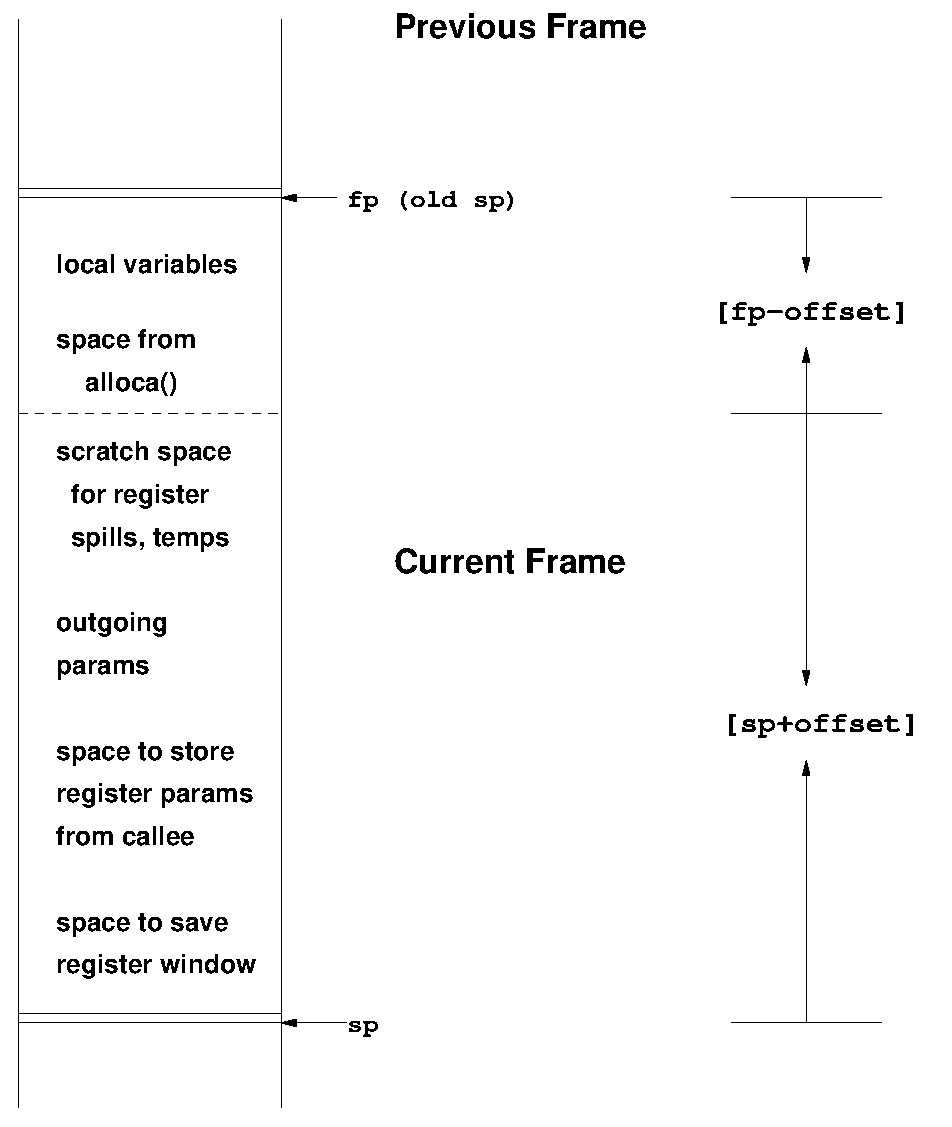
\psfig{file=RISCstack.eps,width=20em}
\end{center}
\vfil
\end{slide*}

\begin{slide*}
Stack frames:
\begin{itemize}
\item stores function activations;
\item {\tt sp} and {\tt fp} point to stack frames;
\item when a function is called a new stack frame is created:\\
      {\tt push fp; fp := sp; sp := sp + C};
\item when a function returns, the top stack frame is popped:\\
      {\tt sp := fp;  fp = pop};
\item local variables are stored relative to {\tt fp};
\item the figure shows additional features of the SPARC architecture.
\end{itemize}
\vfil
\end{slide*}

\begin{slide*}
A simple C function:\\

\begin{tt}
\begin{verbatim}
int fact(int n)
{ int i, sum;
  sum = 1;
  i = 2;
  while (i <= n)
    { sum = sum * i;
      i = i + 1;
    }
  return sum;
}
\end{verbatim}
\end{tt}
\vfil
\end{slide*}

\begin{slide*}
Corresponding VirtualRISC code:\\

\begin{tt}
\begin{scriptsize}
\begin{verbatim}
_fact:
  save sp,-112,sp   // save stack frame
  st R0,[fp+68]     // save input arg n in frame of CALLER
  mov 1,R0          // R0 := 1
  st R0,[fp-16]     // [fp-16] is location for sum
  mov 2,R0          // RO := 2
  st RO,[fp-12]    // [fp-12] is location for i
L3:
  ld [fp-12],R0     // load i into R0
  ld [fp+68],R1     // load n into R1
  cmp R0,R1         // compare R0 to R1
  ble L5            // if R0 <= R1 goto L5
  b L4              // goto L4
L5:
  ld [fp-16],R0     // load sum into R0
  ld [fp-12],R1     // load i into R1
  mul R0,R1,R0      // R0 := R0 * R1
  st R0,[fp-16]     // store R0 into sum
  ld [fp-12],R0     // load i into R0
  add R0,1,R1       // R1 := R0 + 1
  st R1,[fp-12]     // store R1 into i
  b L3              // goto L3
L4:
  ld [fp-16],R0     // put return value of sum into R0
  restore           // restore register window
  ret               // return from function
\end{verbatim}
\end{scriptsize}
\end{tt}
\vfil
\end{slide*}

\begin{slide*}
Java Virtual Machine has:
\begin{itemize}
\item memory;
\item registers;
\item condition codes; and
\item execution unit.
\end{itemize}
\vfil
\end{slide*}

\begin{slide*}
Java Virtual Machine memory:
\begin{itemize}
\item a stack\\(used for function call frames);
\item a heap\\(used for dynamically allocated memory);
\item a constant pool\\(used for constant data that can be shared); and
\item a code segment\\(used to store JVM instructions of currently loaded
                     class files).
\end{itemize}
\vfil
\end{slide*}
 
\begin{slide*}
Java Virtual Machine registers:
\begin{itemize}
\item no general purpose registers;
\item the stack pointer ({\tt sp}) which points to the top of the stack;
\item the local stack pointer ({\tt lsp}) which points to a location in
            the current stack frame; and
\item the program counter ({\tt pc}) which points to the current instruction.
\end{itemize}
\vfil
\end{slide*}

\begin{slide*}
Java Virtual Machine condition codes:
\begin{itemize}
\item stores the result of last instruction that can
       set condition codes (used for branching).
\end{itemize}

Java Virtual Machine execution unit:
\begin{itemize}
\item reads the Java Virtual Machine instruction at the current {\tt pc},
       decodes the instruction and executes it;
\item this may change the state of the machine (memory, registers, condition
 codes);
\item the {\tt pc} is automatically incremented after executing
    an instruction; but
\item method calls and branches explicitly
    change the {\tt pc}.
\end{itemize}
\vfil
\end{slide*}

\begin{slide*}
Java Virtual Machine stack frames have space for:
\begin{itemize}
\item a reference to the current object ({\tt this});
\item the method arguments;
\item the local variables; and
\item a local stack used for intermediate results.
\end{itemize}
The number of local slots and the maximum size of the local stack
are fixed at compile-time.
\vfil
\end{slide*}

\begin{slide*}
Java compilers translate source code to class files.

Class files include the bytecode instructions for each method.\\
~\\

\begin{center}
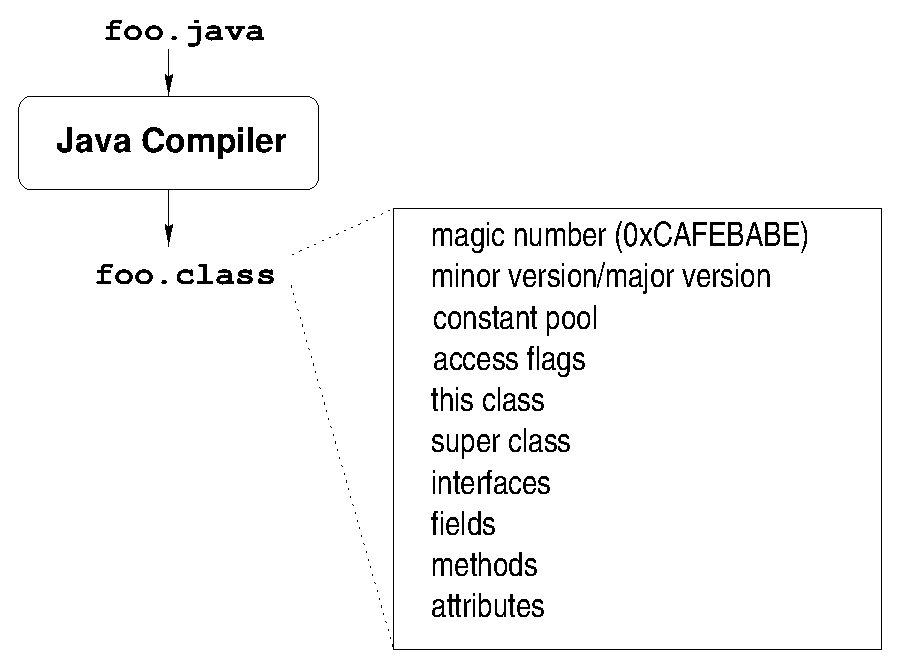
\psfig{file=java2class.eps,width=20em}
\end{center}
\vfil
\end{slide*}

\begin{slide*}
A simple Java method:

\begin{tt}
\begin{verbatim}
public int Abs(int x)
{ if (x < 0)
   return(x * -1);
 else
   return(x);
}
\end{verbatim}
\end{tt}

Corresponding bytecode (in Jasmin syntax):

\begin{tt}
\begin{scriptsize}
\begin{verbatim}
.method public Abs(I)I // one int argument, returns an int
.limit stack 2         // has stack with 2 locations
.limit locals 2        // has space for 2 locals
 
                       // --locals--  --stack---
                       // [ o -3 ]     [  *  * ]
  iload_1              // [ o -3 ]     [ -3  * ]
  ifge Label1          // [ o -3 ]     [  *  * ]
  iload_1              // [ o -3 ]     [ -3  * ]
  iconst_m1            // [ o -3 ]     [ -3 -1 ]
  imul                 // [ o -3 ]     [  3  * ]
  ireturn              // [ o -3 ]     [  *  * ]
Label1:
  iload_1
  ireturn
.end method
\end{verbatim}
\end{scriptsize}
\end{tt}

Comments show trace of {\tt o.Abs(-3)}.
\vfil
\end{slide*}

\begin{slide*}
A sketch of a bytecode interpreter:\\

\begin{tt}
\begin{scriptsize}
\begin{verbatim}
pc = code.start;
while(true)
  {  npc = pc + instruction_length(code[pc]);
     switch (opcode(code[pc]))
       {  case ILOAD_1: push(local[1]);
                        break;
          case ILOAD:   push(local[code[pc+1]]);
                        break;
          case ISTORE:  t = pop();
                        local[code[pc+1]] = t;
                        break;
          case IADD:    t1 = pop();  t2 = pop();
                        push(t1 + t2);
                        break;
          case IFEQ:    t = pop();
                        if (t == 0) npc = code[pc+1];
                        break;
          ...
       }
     pc = npc;
  }
\end{verbatim}
\end{scriptsize}
\end{tt}
\vfil
\end{slide*}

\begin{slide*}
Unary arithmetic operations:\\

\begin{tt}
\begin{tabbing}
XXXXXXXXXXX\=\kill
ineg\>[...:i] -> [...:-i]\\
i2c\>[...:i] -> [...:i\%65536]\\
\end{tabbing}
\end{tt}

Binary arithmetic operations:\\
 
\begin{tt}
\begin{tabbing}
XXXXXXXXXXX\=\kill
iadd\>[...:i1:i2] -> [...:i1+i2]\\
isub\>[...:i1:i2] -> [...:i1-i2]\\
imul\>[...:i1:i2] -> [...:i1*i2]\\
idiv\>[...:i1:i2] -> [...:i1/i2]\\
irem\>[...:i1:t2] -> [...:i1\%i2]\\
\end{tabbing}
\end{tt}

Direct operations:\\

\begin{tt}
\begin{tabbing}
XXXXXXXXXXX\=\kill
iinc k a\>[...] -> [...]\\\>local[k]=local[k]+a\\
\end{tabbing}
\end{tt}
\vfil
\end{slide*}

\begin{slide*}
Nullary branch operations:\\

\begin{tt}
\begin{tabbing}
XXXXXXXXXXXXXX\=\kill
goto L\>[...] -> [...]\\\>{branch always}\\
\end{tabbing}
\end{tt}

Unary branch operations:\\
 
\begin{tt}
\begin{tabbing}
XXXXXXXXXXXXXX\=\kill
ifeq L\>[...:i] -> [...]\\\>{branch if} i == 0\\
ifne L\>[...:i] -> [...]\\\>{branch if} i != 0\\
\\
ifnull L\>[...:o] -> [...]\\\>{branch if} o == null\\
ifnonnull L\>[...:o] -> [...]\\\>{branch if} o != null\\
\end{tabbing}
\end{tt}

\vfil
\end{slide*}

\begin{slide*}
Binary branch operations:\\
 
\begin{tt}
\begin{tabbing}
XXXXXXXXXXXXXX\=\kill
if\_icmpeq L\>[...:i1:i2] -> [...]\\\>{branch if} i1 == i2\\
if\_icmpne L\>[...:i1:i2] -> [...]\\\>{branch if} i1 != i2\\
if\_icmpgt L\>[...:i1:i2] -> [...]\\\>{branch if} i1 > i2\\
if\_icmplt L\>[...:i1:i2] -> [...]\\\>{branch if} i1 < i2\\
if\_icmple L\>[...:i1:i2] -> [...]\\\>{branch if} i1 <= i2\\
if\_icmpge L\>[...:i1:i2] -> [...]\\\>{branch if} i1 >= i2\\
\\
if\_acmpeq L\>[...:o1:o2] -> [...]\\\>{branch if} o1 == o2\\
if\_acmpne L\>[...:o1:o2] -> [...]\\\>{branch if} o1 != o2\\
\end{tabbing}
\end{tt}
 
\vfil
\end{slide*}

\begin{slide*}
Constant loading operations:\\

\begin{tt}
\begin{tabbing}
XXXXXXXXXXXXXX\=\kill
iconst\_0\>[...] -> [...:0]\\
iconst\_1\>[...] -> [...:1]\\
iconst\_2\>[...] -> [...:2]\\
iconst\_3\>[...] -> [...:3]\\
iconst\_4\>[...] -> [...:4]\\
iconst\_5\>[...] -> [...:5]\\
\\
aconst\_null\>[...] -> [...:null]\\
\\
ldc\_int i\>[...] -> [...:i]\\
ldc\_string s\>[...] -> [...:String(s)]\\
\end{tabbing}
\end{tt}
\vfil
\end{slide*}

\begin{slide*}
Locals operations:\\

\begin{tt}
\begin{tabbing}
XXXXXXXXXXXXXXXXX\=\kill
iload k\>[...] -> [...:local[k]]\\
istore k\>[...:i] -> [...]\\
        \>local[k]=i\\
\\
aload k\>[...] -> [...:local[k]]\\
astore k\>[...:o] -> [...]\\
        \>local[k]=o\\
\end{tabbing}
\end{tt}

Field operations:\\

\begin{tt}
\begin{tabbing}
XXXXXXXXXXXXXXXXX\=\kill
getfield f sig\>[...:o] -> [...:o.f]\\
putfield f sig\>[...:o:v] -> [...]\\
              \>o.f=v\\
\end{tabbing}
\end{tt}
\vfil
\end{slide*}

\begin{slide*}
Stack operations:\\

\begin{tt}
\begin{tabbing}
XXXXXXXXXXXX\=\kill
dup    \>[...:v1] -> [...:v1:v1]\\
pop    \>[...:v1] -> [...]\\
swap   \>[...:v1:v2] -> [...:v2:v1]\\
nop    \>[...] -> [...]\\
\end{tabbing}
\end{tt}
\vfil
\end{slide*}

\begin{slide*}
Class operations:\\

\begin{tt}
\begin{tabbing}
XXXXXXXXXXXXXXX\=\kill
new C\>[...] -> [...:o]\\
\\
instance\_of C\>[...:o] -> [...:i]\\
             \>if (o==null) i=0\\
             \>else i=(C<=type(o))\\
\\
checkcast C\>[...:o] -> [...:o]\\
           \>if (o!=null \&\& !C<=type(o))\\
           \>throw ClassCastException\\
\end{tabbing}
\end{tt}
\vfil
\end{slide*}

\begin{slide*}
Method operations:\\
 
\begin{tt}
\begin{tabbing}
XXXXXXXXXXXXXXX\=\kill
invokevirtual m sig\\
~~~~~[...:o:a$_1$:...:a$_n$] -> [...]\\
\\
//overloading already resolved:\\
//   signature of m is known!\\
entry=lookup\underbar{Hierarchy}(m,sig,class(o));\\
block=block(entry);\\
push stack frame of size\\
~~~~~block.locals+block.stacksize;\\
local[0]=o; //local points to\\
local[1]=a$_1$;  //beginning of frame\\
...\\
local[n]=a$_n$;\\
pc=block.code;\\
\end{tabbing}
\end{tt}
\vfil
\end{slide*}

\begin{slide*}
Method operations:\\
 
\begin{tt}
\begin{tabbing}
XXXXXXXXXXXXXXX\=\kill
invokespecial m sig\\
~~~~~[...:o:a$_1$:...:a$_n$] -> [...]\\
\\
//overloading already resolved:\\
//   signature of m is known!\\
entry=lookup\underbar{ClassOnly}(m,sig,class(o));\\
block=block(entry);\\
push stack frame of size\\
~~~~~block.locals+block.stacksize;\\
local[0]=o; //local points to\\
local[1]=a$_1$;  //beginning of frame\\
...\\
local[n]=a$_n$;\\
pc=block.code;\\
\end{tabbing}
\end{tt}
For which method calls is {\tt invokespecial} used?
%%ANSWER:
%<init>(..) calls
%private method calls
%super-method calls
\vfil
\end{slide*}

\begin{slide*}
Method operations:\\
 
\begin{tt}
\begin{tabbing}
XXXXXXXXXXXX\=\kill
ireturn  \>[...:<frame>:i] -> [...:i]\\
         \>pop stack frame,\\
         \>push i onto frame of caller\\
\\
areturn  \>[...:<frame>:o] -> [...:o]\\
         \>pop stack frame,\\
         \>push o onto frame of caller\\
\\
return   \>[...:<frame>] -> [...]\\
         \>pop stack frame
\end{tabbing}
\end{tt}
\bigskip
Those operations also release locks in {\tt synchronized} methods.
\vfil
\end{slide*}

\begin{slide*}
A Java method:\\
 
\begin{verbatim}
public boolean member(Object item)
{ if (first.equals(item))
    return true;
  else if (rest == null)
    return false;
  else
    return rest.member(item);
}
\end{verbatim}
\vfil
\end{slide*}

\begin{slide*}
Corresponding bytecode (in Jasmin syntax):\\
\begin{scriptsize}
\begin{verbatim}
.method public member(Ljava/lang/Object;)Z
.limit locals 2            // local[0] = o
                           // local[1] = item
.limit stack 2             // initial stack [ * * ]
aload_0                    // [ o * ]
getfield Cons/first Ljava/lang/Object;     
                           // [ o.first *]
aload_1                    // [ o.first item]
invokevirtual java/lang/Object/equals(Ljava/lang/Object;)Z 
                           // [ b * ] for some boolean b 
ifeq else_1                // [ * * ]
iconst_1                   // [ 1 * ]
ireturn                    // [ * * ]
else_1:
aload_0                    // [ o * ]
getfield Cons/rest LCons;  // [ o.rest * ]
aconst_null                // [ o.rest null]
if_acmpne else_2           // [ * * ]
iconst_0                   // [ 0 * ]
ireturn                    // [ * * ]
else_2:
aload_0                    // [ o * ]
getfield Cons/rest LCons;  // [ o.rest * ]
aload_1                    // [ o.rest item ]
invokevirtual Cons/member(Ljava/lang/Object;)Z  
                           // [ b * ] for some boolean b 
ireturn                    // [ * * ]
.end method
\end{verbatim}
\end{scriptsize}
\vfil
\end{slide*}


\begin{slide*}
Bytecode verification:
 
\begin{itemize}
\item bytecode cannot be trusted to be
well-formed and well-behaved;
\item before executing any bytecode, it
should be verified, especially if that bytecode is received over the network;
\item verification is performed partly
at class loading time, and partly at
run-time; and
\item at load time, dataflow
analysis is used to approximate the
number and type of values in locals
and on the stack.
\end{itemize}
\vfil
\end{slide*}

\begin{slide*}
Interesting properties of verified bytecode:
 
\begin{itemize}
\item each instruction must be executed
with the correct number and types of arguments
on the stack, and in locals (on all execution
paths);
\item at any program point, the stack is
the same size along all execution paths;
\item every method must have enough locals to hold
the receiver object (except static methods) and the method's arguments; and
\item
no local variable can be accessed before it
has been assigned a value.
\end{itemize}
\vfil
\end{slide*}

\begin{slide*}
Java class loading and execution model:
\begin{itemize}
\item when a method is invoked,  a {\tt ClassLoader}
finds the correct class and checks that it contains an
appropriate method;
\item if the method has not yet been
loaded, then it is verified (remote classes); 
\item
after loading and verification, the method body is interpreted.
\item If the method becomes executed multiple times, the bytecode for that
method is translated to native code.
\item If the method becomes hot, the native code is optimized.
\end{itemize}
The last two steps are very involved and companies like Sun and IBM have
a thousand people working on optimizing these steps.

\hfill $\Rightarrow$ good for you! (why not 1001 people?)
\vfil
\end{slide*}

\begin{slide*}
Split-verification in Java 6+:
\begin{itemize}
  \item Bytecode verification is easy but still polynomial, i.e. sometimes slow,
  and
  \item this can be exploited in denial-of-service attacks:
		\url{http://www.bodden.de/research/javados/}
  \item
	Java 6 (version 50.0 bytecodes) introduced {\tt StackMapTable} attributes to
	make verification linear.
  \begin{itemize}
    \item Java compilers know the type of locals at compile time.
    \item Java 6 compilers store these types in the bytecode using {\tt
    StackMapTable} attributes.
    \item Speeds up construction of the ``proof tree'' $\Rightarrow$ also
    called ``Proof-Carrying Code''
  \end{itemize}
  \item Java 7 (version 51.0 bytecodes) JVMs will enforce presence of these
 attributes.
\vfil
   
\end{itemize}
\end{slide*}


\begin{slide*}
Future use of Java bytecode:
\begin{itemize}
\item
the JOOS compiler will produce Java bytecode in
                   Jasmin format; and
\item the JOOS peephole optimizer transforms bytecode into
                   more efficient bytecode.
\end{itemize}

Future use of VirtualRISC:
\begin{itemize}
\item
Java bytecode can be converted into machine code
                  at run-time using a JIT (Just-In-Time) compiler;
\item
we will study some examples of converting Java bytecode
                  into a language similar to VirtualRISC;
\item
we will study some
                  simple, standard optimizations on VirtualRISC.
\end{itemize}
\vfil
\end{slide*}


\end{document}
